% Created 2016-05-31 mar. 12:08
\documentclass[a4paper]{article}
\usepackage[utf8]{inputenc}
\usepackage[T1]{fontenc}
 \usepackage{lmodern}
\usepackage{fixltx2e}
\usepackage{graphicx}
\usepackage{longtable}
\usepackage{float}
\usepackage{wrapfig}
\usepackage{rotating}
\usepackage[normalem]{ulem}
\usepackage{amsmath}
\usepackage{textcomp}
\usepackage{marvosym}
\usepackage{wasysym}
\usepackage{amssymb}
\usepackage{hyperref}
\hypersetup{
colorlinks=true,
linkcolor=blue,
pdfauthor=Simon Gascoin,
pdftitle=Algorithm theoretical basis documentation for an operational snow cover product from Sentinel-2 and Landsat-8 data (Let-it-snow)}
\tolerance=1000
\usepackage{amsfonts,bm}
\usepackage{color}
\usepackage[usenames,dvipsnames]{xcolor}
\usepackage[margin=2.5cm,a4paper]{geometry}
\usepackage{enumitem}
\usepackage[]{algorithm2e}
\usepackage{fancyhdr}
\usepackage{tabularx}
%\usepackage{listings}
\usepackage{minted}
% \lstset{language=Matlab}

\usepackage{tikz}
\usetikzlibrary{shapes,arrows,decorations.markings,shapes,fit}


\renewcommand{\maketitle}{}
\date{\today}
% \title{ATBD CES surface enneigée}
% \hypersetup{
%   pdfkeywords={},
%   pdfsubject={},
%   pdfcreator={Emacs 24.3.1 (Org mode 8.2.4)}}
\begin{document}

\maketitle
\pagestyle{fancy}
% \providecommand{\alert}[1]{\textbf{#1}}
% \setlist[itemize,1]{label=$\diamond$}
% \setlist[itemize,2]{label=$\ast$}
% \setlist[itemize,3]{label=$\star$}
% \setlist[itemize,4]{label=$\bullet$}
% \setlist[itemize,5]{label=$\circ$}
% \setlist[itemize,6]{label=$-$}
% \setlist[itemize,7]{label=$\cdot$}
% \setlist[itemize,8]{label=$\cdot$}
% \setlist[itemize,9]{label=$\cdot$}
% \renewlist{itemize}{itemize}{9}
\lhead[]{
\includegraphics[width=0.1\textwidth]{./images/logo_cesbio.png}}
\rhead[]{\thepage}
% \cfoot{\textcolor{PineGreen}{copyright?}}

\begin{titlepage}

\includegraphics[width=0.3\textwidth]{./images/logo_cesbio.png}
\hspace{5cm}

\includegraphics[width=0.3\textwidth]{./images/Theia_en.png}

\vspace{3cm}



\textcolor{PineGreen}{ \huge \bfseries Theia Land Data Centre\\ }
% \vspace{0.5cm}
\rule{\linewidth}{0.5mm}
\begin{center}
{ \huge \bfseries Algorithm theoritical basis documentation for an operational snow cover extent product from Sentinel-2 and Landsat-8 data (Let-it-snow)\\}
\rule{\linewidth}{0.5mm}
{ \large \bfseries Simon Gascoin (CNRS/CESBIO), Manuel Grizonnet (CNES/CT/DSI), Tristan Klempka (CNES/CT/DSI)\\ }
{ \large \bfseries V1.0 (Updated for LIS 1.2) - \today \\ }

% \vspace{3cm}
% 
\includegraphics[width=1\textwidth]{./Images/Theia_en.png}


\end{center}
\end{titlepage}


\begin{abstract}
 
This document describes the algorithm of the Let-it-snow (LIS) processing chain to generate the snow cover extent product for the Theia land data center. The algorithm takes as input a Sentinel-2 or Landsat-8 image of surface reflectance corrected from atmospheric and slope effects, the associated cloud mask (level 2A product provided by Theia) and a digital elevation model. The output is a single band raster at the same resolution of the input image giving the snow presence or absence and a cloud mask. The output cloud mask is different from the input cloud mask because some pixels can be reclassified as snow or no-snow by the algorithm.

The snow detection algorithm works in two passes: first the most evident snow cover is detected using a set of conservative thresholds, then these snow pixels are used to determine the lowest elevation of the snow cover. A second pass is performed for the pixels above this elevation with a new set of less conservative thresholds.

The processing chain also generates a vectorized version of the snow mask after pass 1 and 2 and a color composite that is overlaid by these polygons. These secondary products are intended for expert validation purpose.

\end{abstract}

\newpage
\tableofcontents
\newpage
% 
\section{Introduction}\label{par:intro}

\subsection{Motivation}

The snow cover is a key factor of many ecological, climatological and hydrological processes in cold regions. The monitoring of the snow cover is of particular societal relevance in mountain regions since the seasonal snow melt modifies the soil moisture, groundwater recharge and river flow, often providing critical water resources to downstream areas\footnote{Barnett T. P., Adam J. C. and Lettenmaier D. P., Potential impacts of a warming climate on water availability in snow-dominated regions, Nature 438 (7066), 2005.}. 

The snow cover is one of the 50 Essential Climate Variables (ECVs) that were defined by the Global Observing System for Climate (GCOS)\footnote{GCOS Essential Climate Variables  \url{http://www.wmo.int/pages/prog/gcos/index.php?name=EssentialClimateVariables}} in accordance with the Committee on Earth Observation Satellites (CEOS) agencies\footnote{Global Climate Observing System (GCOS) Implementation Plan \url{http://remotesensing.usgs.gov/ecv/document/gcos-138.pdf}} to support the work of the UNFCCC and the IPCC. 

The \textit{snow cover extent} or \textit{snow cover area} is the extent of the snow cover on the land surface. A snow cover extent product is typically formatted as a georeferenced raster image whose pixel value indicate if snow is present or absent in the pixel.

Other major satellite snow products include: (i) the snow cover fraction (ii) snow albedo (iii) the snow water equivalent. The snow cover fraction and albedo are generated from optical observations, while the snow water equivalent is retrieved using passive or active microwave. The snow water equivalent is potentially the most useful product since it gives directly the amount of accumulated water (snow mass), however current products are unsuitable to address user needs for many applications and places because they are available at coarse scale (25~km) with some limitations in the retrievals. This is due to the lack of observations in the wavelengths that are adapted to snow water equivalent sensing. As of today the snow cover extent product is still the most widely used for hydrological and climatological applications. This will certainly remain true for the next decade since there is no planned mission to retrieve the snow water equivalent or the snow depth at global scale\footnote{This was the objective of the CoreH2O mission but the project was not selected by the ESA for the Earth Explorer-7 program in 2015.}. 

Current snow cover area products are derived from low to mid-resolution optical observations (e.g. AVHRR, VEGETATION, MODIS) but their spatial resolution (1~km to 250~m) is too coarse for various applications, in particular in mountain regions where the topography causes large spatial variability of the snow cover at decametric scales. High resolution snow cover maps can be generated from Landsat images but the temporal revisit of 16~days is not sufficient for snow cover monitoring during the melt season. The ESA Sentinel-2 mission offers the unique opportunity to study the snow cover extent dynamics at 20 m resolution with a 5 day revisit time. If combined with Landsat the temporal resolution can be further increased. Both Sentinel-2 and Landsat missions are global missions that are expected to run over long periods, allowing the development of operational products and services\footnote{Drusch M., Del Bello U., Carlier S. et al., Sentinel-2: ESA's Optical High-Resolution Mission for GMES Operational Services, Remote Sensing of Environment 120, 2012.}.

\subsection{Objective}

The objective of this algorithm is to generate a snow cover extent product from Landsat-8 and Sentinel-2 images at high resolution (30~m for Landsat-8, 20~m for Sentinel-2). The main requirements are:
\begin{itemize}
 \item The algorithm should be efficient to allow the processing of large areas (10$^4$ km$^2$) with a reasonable computation cost. 
 \item It should be robust to seasonal and spatial variability of the snow cover and land surface properties. 
 \item It should maximize the number of pixels that are classified as snow or no-snow.
 \item It is always preferable to falsely classify a pixel as cloud than falsely classify a pixel as snow or no-snow. 
%  \item It should not depend on uncertain external data (like meteorological data) to limit the risk of a product discontinuation.
\end{itemize}

\subsection{Development}

The algorithm prototype was developed by Simon Gascoin with insights from Olivier Hagolle in June 2015.  The snow detection function and a script to run this function with an example are given in appendices \ref{par:castest} and \ref{par:s2snow} as formatted documents that includes the original Matlab code, comments, and output. The LIS chain was designed to work on any high resolution multi-spectral images from satellite sensors that include at least a channel in the visible spectrum and a channel near 1.5 µm (typically referred to as mid-infrared or ``MIR''). This initial code was ported to Python 2.7 and C++ by Manuel Grizonnet in order to make it scalable to large images using Orfeo Toolbox and GDAL. The LIS code was enhanced by Tristan Klempka during his internship at CNES. LIS currently supports SPOT-4, SPOT-5, Landsat-8 and Sentinel-2 level 2A products. The LIS code, installation documentation and configuration file examples are available in the Cesbio's gitlab: \url{http://tully.ups-tlse.fr/grizonnet/let-it-snow}. 

\subsection{Limitations}

The product is based on optical observations therefore it is not adapted to the detection of the snow cover:

\begin{itemize}
 \item in polar regions when illumination is insufficient ;
  \item in dense forest areas where the ground is obstructed by the canopy, like in evergreen conifer forests.
 \end{itemize}
 
The algorithm may also fail to detect the snow cover in steep shaded slopes if the solar elevation is very low (typically below 20°). This can occur in mid-latitude areas in winter. In this case the slope correction in the L2A product is generally not applied as indicated in the L2A mask.

The algorithm can only reduce the number of cloud pixels from the original L2A cloud mask. If a cloud was not detected by the previous cloud mask algorithm (MACCS) then it can only be classified as snow or no-snow. 

The algorithm output depends on the scale of the input because the snowline elevation is computed at the scale of the image. In the case of the level 2A products this is 110~km by 110~km. The underlying assumption is that a large altitudinal variation of the snowline elevation is not likely at such a scale. Our impression is that this assumption is supported by regional analyses of the snowline in many mountain ranges, but this could be further assessed using mid-resolution snow products\footnote{Gascoin, S., Hagolle, O., Huc, M., Jarlan, L., Dejoux, J.-F., Szczypta, C., Marti, R., and Sánchez, R.: A snow cover climatology for the Pyrenees from MODIS snow products, Hydrol. Earth Syst. Sci., 19, 2337-2351}\footnote{Krajčí P., Holko L. and Parajka J., Variability of snow line elevation, snow cover area and depletion in the main Slovak basins in winters 2001–2014, Journal of Hydrology and Hydromechanics 64(1), 2016}.

\section{Algorithm}\label{par:algo}

\subsection{Inputs}\label{par:inputs}
\begin{itemize}
 \item From a level 2A product:
 \begin{itemize}
  \item the cloud and cloud shadow mask (referred to as ``L2A cloud mask'' in the following),
  \item the green, red and MIR bands from the flat surface reflectance product (Tab.~\ref{tab:bands}). These images are corrected for atmospheric and terrain slope effects. The slope correction is important in mountain regions since it enables to use the same detection thresholds whatever the sun-slope geometry. 
  \end{itemize}
  \item A digital elevation model (DEM). The DEM is resampled from the SRTM seamless DEM\footnote{Jarvis A., H.I. Reuter, A.  Nelson, E. Guevara, 2008, Hole-filled  seamless SRTM data V4, International  Centre for Tropical  Agriculture (CIAT), available  from \url{http://srtm.csi.cgiar.org}.}. 
  \item The parameters of the algorithm: \textcolor{red}{$r_f$, $d_z$, $r_B$, $r_D$, ,$n_1$, $n_2$, $r_1$, $r_2$, $f_s$, $f_t$} (written \textcolor{red}{in red} throughout the document).
  
\end{itemize}

\begin{table}[h]
\begin{center}
\begin{tabular}{|l|lll|}
\hline
  & \multicolumn{3}{|c|}{Band}\\
\hline
Sensor & Green & Red & MIR\\
\hline
SPOT-4 HRV & 1 (20 m, 0.55 µm) & 2 (20 m, 0.65 µm) & 4 (20~m, 1.6 µm)\\
SPOT-5 HRG & 1 (10 m, 0.55 µm) & 2 (10 m, 0.65 µm) & 4 (10~m, 1.6 µm)\\
Sentinel-2 MSI & 2 (10 m, 0.56 µm) & 3 (10 m, 0.66 µm) & 5 (20 m, 1.6 µm)\\
Landsat-8 OLI & 3 (30 m, 0.56 µm) & 4 (30 m, 0.65 µm) & 6 (30 m, 1.6 µm)\\
\hline
\end{tabular}
\end{center}
\caption{Index of the spectral band in the L2A flat surface reflectance products used by LIS. In parentheses is also indicated the spatial resolution and the wavelength of the band center.}
\end{table}\label{tab:bands}

\subsection{Outputs}\label{par:outputs}

The main output is a raster image (*SEB.TIF) of the snow and cloud mask. It has the same projection and extent of the initial L2A product and the same resolution as the MIR band, i.e. 20~m for Sentinel-2 and SPOT-4, 30~m for Landsat-8 (Tab.~\ref{tab:bands}). It coded as follows:
\begin{itemize}
 \item 0: no-snow
 \item 100: snow
 \item 205: cloud including cloud shadow
 \item 254: no data
\end{itemize}

The same data are made available as a polygon shapefile of the cloud and snow cover extent (*SEB\_VEC*). Two fields of information are embedded in this file:
\begin{itemize}
  \item DN:
  \begin{itemize}
    \item 0: no-snow
    \item 100: snow
    \item 205: cloud including cloud shadow
    \item 254: no data
  \end{itemize}
  \item field:
  \begin{itemize}
    \item no-snow
    \item snow
    \item cloud
    \item no-data
  \end{itemize}
\end{itemize}

The other output files are rather useful for the expert evaluation and troubleshooting:
\begin{itemize}
 \item an RGB color composite image of bands MIR/red/green also showing the snow and cloud mask boundaries (*COMPO.TIF);
 \item a binary mask of snow and clouds (*SEB\_ALL.TIF):
 \begin{itemize}
 \item bit 1: snow (pass 1)
 \item bit 2: snow (pass 2)
 \item bit 3: clouds (pass 1)
 \item bit 4: clouds (pass 2)
 \end{itemize}
 \item a metadata file (*METADATA.XML)
 
\end{itemize}

\subsection{Pre-processing}

In the case of Sentinel-2 the red and green bands are first resampled with the cubic method to a pixel size of 20~m by 20~m to match the resolution of the MIR band.

The DEM is also resampled to the resolution of the target product (30~m or 20~m, see Sect.~\ref{par:outputs}) using the cubic spline method that is implemented in the gdal library.

\subsection{Snow detection}\label{par:snowdetec}

The snow detection is based on the Normalized Difference Snow Index (NDSI) and the reflectance in the red band. The NDSI is defined as\footnote{Dozier, J.: Spectral signature of alpine snow cover from the Landsat Thematic Mapper, Remote sensing of Environment 28, 9–22, 1989}:

\begin{equation}
\mathrm{NDSI} = \frac{\rho_\mathrm{green}-\rho_\mathrm{MIR}}{\rho_\mathrm{green}+\rho_\mathrm{MIR}}
\end{equation}
where $\rho_\mathrm{green}$ (resp. $\rho_\mathrm{MIR}$) is the slope-corrected surface reflectance in the green band (resp. MIR at 1.6~$\mu$m). The NDSI is based on the fact that only snow surfaces are very bright in the visible but dark in the shortwave infrared. Some lake pixels may also have a high NDSI value so we add a criterion on the red reflectance to remove these. A pixel is classified as snow if the two following conditions are fulfilled:
\begin{itemize}
 \item $\mathrm{NDSI} > n_i$,
 \item $\rho_\mathrm{red} > r_i$
\end{itemize}
where $n_i$ and $r_i$ are two parameters with $i=\{1,2\}$. Otherwise the pixel is marked as no-snow. 


\subsection{Snowline elevation}

The snow detection (Sect.~\ref{par:snowdetec}) is performed a first time using thresholds \textcolor{red}{$n_1$} and \textcolor{red}{$r_1$}. The parameters are set to low values to minimize the false snow detections. As a consequence, many snow covered areas are not detected. However, this pass 1 enables to estimate a minimum snow cover elevation $z_s$. For that purpose the DEM is used to segment the image in elevation band of height \textcolor{red}{$d_z$}. The fraction of the cloud-free area of each band that is covered by snow is computed. We find the lowest elevation band $b$ at which the the snow cover fraction is greater than \textcolor{red}{$f_s$}. Then, $z_s$ is defined as the lower edge of the elevation band that is two elevation bands below band $b$. The snow cover fraction in each elevation band is determined using the pixels that are not marked as cloud in the pass 1 cloud mask (Sect.~\ref{par:cloud}). To ensure that $z_s$ is computed with a statistically significant sample of pixels, the snowline calculation is not activated if the total fraction of snow pixels in the image is lower than $f_t$. A detailed example of the determination of $z_s$ is given in appendix~\ref{par:castest}.

\subsection{Cloud mask processing}\label{par:cloud}

The L2A cloud mask is conservative because it is computed at a coarser resolution and also because it is developed for a large range of applications. However, the detection of the snow cover is robust to a thin, transparent, cloud cover. More importantly, the L2A cloud mask tends to falsely classify the edges of the snow cover as cloud. Hence, it is possible to recover many pixels from the L2A cloud mask and reclassify them as snow or no-snow. This step is important because it substantially increases the number of observations. A pixel from the L2A cloud mask cannot be reclassified as snow or no-snow if:

\begin{itemize}
 \item it is coded as ``cloud shadow''  in L2A cloud mask. Note that it can be
   cloud shadows matched with a cloud or cloud shadows in the zone where clouds could be outside the image ;
 \item or: it is coded as ``high altitude cloud'' (or ``cirrus'') in the L2A cloud mask;
 \item or: it is not a ``dark'' cloud (see below).
\end{itemize}

The cloud shadows are excluded because the signal-to-noise ratio is too low in these areas. 

The ``high clouds'' are excluded because they can have a similar spectral signature as the snow cover (high reflectance in the visible and low reflectance in the MIR). This type of cloud is only detected in Landsat-8 and Sentinel-2 images because it is based on the spectral band centered on the 1.38 µm wavelength\footnote{Hagolle, O., High cloud detection using the cirrus band of LANDSAT 8 or Sentinel-2, \url{http://www.cesbio.ups-tlse.fr/multitemp/?p=4109}}, therefore the test is not activated for SPOT images.

We select only the ``dark clouds'' because the snow test is robust to the snow/cloud confusion in this case. The ``dark'' clouds are defined using a threshold in the red band after down-sampling the red band by a factor \textcolor{red}{$r_f$} using the bilinear method. This resampling is applied to smooth locally anomalous pixels\footnote{It was also inspired by the MACCS algorithm, which performs the cloud detection at 240~m for Landsat-8 L2A products.}. Therefore, if a (non-shadow, non-high-cloud) cloud pixel has a red reflectance at this coarser resolution that is lower than $r_D$ then it is temporarily removed from the cloud mask and proceeds to the snow test. The new cloud mask at this stage is the pass 1 cloud mask (Fig.~\ref{fig:flowchart}). 

After passing the pass 1 and 2 snow tests, some pixels that were originally marked as cloud will not be reclassified as snow. These pixels are marked as cloud if they have a reflectance in the red that is greater than $r_B$. Otherwise they are classified as no-snow. Here the full resolution red band is used. The resulting cloud mask is the pass 2 cloud mask. 

\pagestyle{empty}

% Define block styles
\tikzstyle{decision} = [diamond, draw, fill=gray!20, 
    text width=4.5em, text centered, inner sep=0pt]
\tikzstyle{block} = [rectangle, draw, fill=gray!20, 
    text width=5em, text centered, rounded corners, minimum height=4em]
\tikzstyle{blockfinal} = [rectangle, draw, fill=green!20, 
    text width=5em, text centered, rounded corners, minimum height=4em]
\tikzstyle{blockinput} = [rectangle, draw, fill=blue!20, 
    text width=5em, text centered, rounded corners, minimum height=4em]
\tikzstyle{line} = [draw, -latex']
\tikzstyle{cloud} = [draw, ellipse, fill=red!20, node distance=3cm,
    minimum height=2em]
\tikzstyle{bigbox}=[inner sep=20pt]

\begin{figure}[H]
 
\begin{tikzpicture}[node distance = 3.5cm, auto]
    % Place nodes
    \node [blockinput, text width=13em] (Level 2A product) {Level 2A product \begin{itemize}
\item cloud mask 
\item flat surface reflectances (green, red, MIR)
\end{itemize} };
    \node [cloud, left of=Level 2A product, node distance = 6cm] (MUSCATE) {MUSCATE};
%     \node [rectangle, draw, text at top, right of=Level 2A product, node distance = 6cm, minimum height=5em, text width=18em] (leg) {Legend};
    \node [blockfinal, right of=Level 2A product, node distance = 6cm, minimum height=2em, text width=3em] (blockfinalleg) {Output};
    \node [blockinput, left of=blockfinalleg, node distance = 1.5cm, minimum height=2em, text width=3em] (blockinputleg) {Input};
    \node [block, right of=blockfinalleg, node distance = 1.9cm, minimum height=2em] (blockleg) {\textcolor{red}{Parameter}};
    \node[bigbox, fit=(blockinputleg)(blockfinalleg)(blockleg)] (leg) {};
    \node[below right] at (leg.north west) {Legend};
    \node [blockinput, below of=MUSCATE] (DEM) {DEM};
    \node [decision, below of=Level 2A product] (is cloud or shadow?) {Is cloud or shadow?};
    \node [decision, right of=is cloud or shadow?] (darkcloud) {Is shadow or high or bright cloud? \textcolor{red}{$r_D$}};
    \node [blockfinal, right of=darkcloud] (cloudfinal1) {Cloud (pass 1)};
    \node [decision, below of=is cloud or shadow?] (snowtest1) {Is snow? \textcolor{red}{$n_1$}, \textcolor{red}{$r_1$}};
    \node [blockfinal, left of=snowtest1] (pass1) {Snow\\(pass 1)};
    \node [decision, below of=snowtest1] (snowlim) {Enough snow?\\ \textcolor{red}{$f_t$}};
    \node [decision, below of=snowlim] (abovezs) {Is above snowline?};
    \node [block, left of=abovezs] (zs) {Snowline elevation \textcolor{red}{$d_z$}, \textcolor{red}{$f_s$}};       
    \node [decision, right of=abovezs] (snowtest2) {Is snow? \textcolor{red}{$n_2$}, \textcolor{red}{$r_2$}};
    \node [blockfinal, right of=snowtest2] (pass2) {Snow\\(pass 2)};
    \node [decision, below of=snowtest2] (wascloud) {Was cloud?};
	\node [blockfinal, right of=wascloud] (nosnow) {No snow};
    \node [decision, below of=wascloud] (backtocloud) {Is dark? \textcolor{red}{$r_B$}};
    \node [blockfinal, left of=backtocloud] (cloudfinal) {Cloud (pass 2)};

    % Draw edges
    \path [line] (Level 2A product) -- (is cloud or shadow?);
    \path [line,dashed] (MUSCATE) -- (Level 2A product);
    \path [line] (is cloud or shadow?) -- node[near start]{yes} (darkcloud);
    \path [line] (is cloud or shadow?) -- node[near start]{no} (snowtest1);
    \path [line] (darkcloud) -- node[near start]{yes}(cloudfinal1);
    \path [line] (darkcloud) |- node[near start]{no}(snowtest1);
    \path [line] (snowtest1) -- node[near start]{yes} (pass1);
    \path [line] (snowtest1) -- node[near start]{yes} (snowlim);
    \path [line] (snowlim) -- node[near start]{yes} (abovezs);
    \path [line] (abovezs) -- node[near start]{yes} (snowtest2);
    \path [line] (snowtest2) -- node[near start]{yes} (pass2);
    \path [line] (snowtest2) -- node[near start]{no} (wascloud);
    \path [line,dashed] (pass1) -- (zs);
    \path [line,dashed] (zs) -- (abovezs);
    \path [line] (abovezs) |- node[near start]{no} (wascloud);
    \path [line,dashed] (MUSCATE) -- (DEM);
    \path [line,dashed] (DEM) |- (zs);
    \path [line] (wascloud) -- node[near start]{no} (nosnow);
    \path [line] (wascloud) -- node[near start]{yes} (backtocloud);
    \path [line] (backtocloud) -| node[near start]{yes} (nosnow);
    \path [line] (backtocloud) -- node[near start]{no} (cloudfinal);
    
\end{tikzpicture}
\caption{Flowchart of the snow detection algorithm}
\end{figure}\label{fig:flowchart}

\subsection{Parameters description}\label{par:param}

\subsubsection{Main algorithm parameters}\label{par:sciparam}

The table below gives the description of the main parameters of the algorithm:

\begin{table}[!htbp]
\begin{center}
\begin{tabularx}{\textwidth}{|l X l l|}
\hline
Parameter & Description & Name in the configuration file & Default value\\
\hline
\textcolor{red}{$r_f$} & Resize factor to produce the down-sampled red band & \texttt{rf} & 8 for L8 (12 for S2) \\
\textcolor{red}{$r_D$} & Maximum value of the down-sampled red band reflectance to define a dark cloud pixel & \texttt{rRed\_darkcloud} & 0.650 \\
\textcolor{red}{$n_1$} & Minimum value of the NDSI for the pass 1 snow test & \texttt{ndsi\_pass1} & 0.400\\
\textcolor{red}{$n_2$} & Minimum value of the NDSI for the pass 2 snow test & \texttt{ndsi\_pass2} & 0.150\\
\textcolor{red}{$r_1$} & Minimum value of the red band reflectance the pass 1 snow test  & \texttt{rRed\_pass1} & 0.200 \\
\textcolor{red}{$r_1$} & Minimum value of the red band reflectance the pass 2 snow test  & \texttt{rRed\_pass2} & 0.120 \\
\textcolor{red}{$d_z$} & Minimum snow fraction in an elevation band to define $z_s$ & \texttt{fsnow\_lim} & 0.100 \\
\textcolor{red}{$f_t$} & Minimum snow fraction in an elevation band to define $z_s$ & \texttt{fsnow\_lim} & 0.100 \\
\textcolor{red}{$f_s$} & Minimum snow fraction in the image to activate the pass 2 snow test & \texttt{fsnow\_total\_lim} & 0.001 \\
\textcolor{red}{$r_B$} & Minimum value of the red band reflectance to return a non-snow pixel to the cloud mask & \texttt{rRed\_backtocloud} & 0.100 \\
\hline
\end{tabularx}
\end{center}
\caption{LIS algorithm parameters description and default values.}
\end{table}\label{tab:param}

Above default values related to reflectance are given as float values between 0
and 1. Threshold related to reflectance values follow the convention of
considering milli-reflectance as input (values between 0 and 1000) in the json
file. Some products can encode reflectance with other convention (floating
values between 0 and 1 or reflectance between 0 and 10000), to handle those
cases, there is a parameter 'multi' in the json configuration file which allows
to scale reflectance parameters. For instance, for products with reflectance
between 0 and 10000 you can use

\subsubsection{JSON schema of configuration file}\label{par:jsonparam}

The JSON Schema here describes the parameter file format and provide a clear, human-
and machine-readable documentation of all the algorithm parameters. JSON schema
was generated on \href{https://jsonschema.net} with the following options (with
metada and relative id).

\inputminted[tabsize=2, fontsize=\tiny]{js}{schema.json}

\section{Validation}\label{par:validation}

The snow maps derived from Landsat data were generally considered as ``ground truth'' to validate and calibrate lower resolution snow cover products\footnote{Hall, D.K., Riggs, G.A.: Accuracy assessment of the MODIS snow products, Hydrological Processes 21(12), 1534–1547, 2007}. There is no space-borne sensor with a MIR channel that provides higher resolution imagery than Sentinel-2 or Landsat-8. As a consequence it is difficult to conduct a quantitative assessment. Hence the validation of the algorithm and the adjustment of the parameters was primarily done by visual inspection of the snow cover mask boundaries on the color composite images in Moroccan Atlas, Pyrenees, and the French Alps. First tests were done on subsets of SPOT-4 Take~5 images. The Python/C++ implementation of LIS allowed the processing and inspection of larger datasets such as a series of full 57 Landsat-8 scenes over the Pyrenees available from THEIA.

\begin{figure}[h]
 \centering
 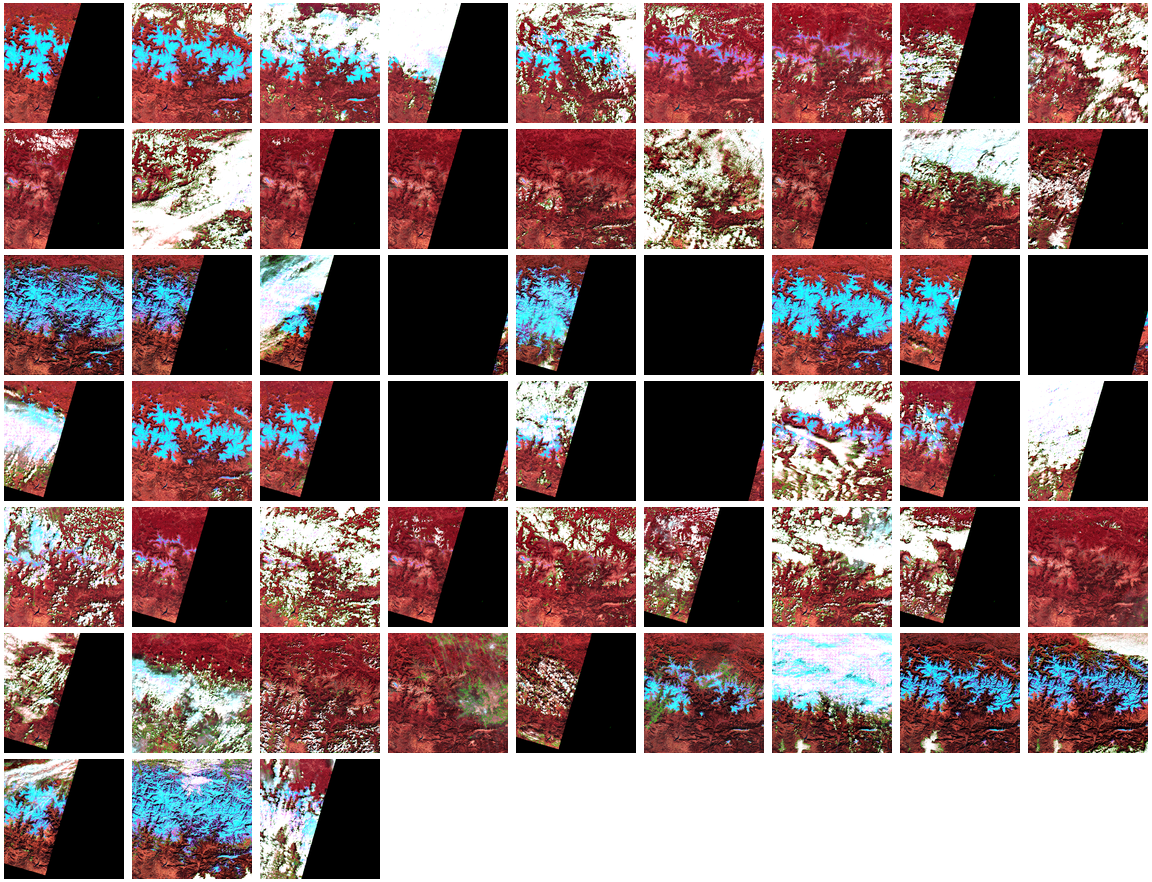
\includegraphics[width=\textwidth]{./images/montage_L8CESneige.png}
 % montage_L8CESneige.png: 1152x882 pixel, 72dpi, 40.64x31.11 cm, bb=0 0 1152 882
 \caption{Color composites of a Landsat-8 tile D0005H0001 time series over the Pyrenees processed by LIS. The snow mask is drawn in magenta and cloud mask in green. Each image is 110 km by 110 km.}
 \label{fig:L8montage}
\end{figure}

The implementation of the Sentinel-2 configuration was tested on the Sentinel-2A image of 06-July-2015 tile 30TYN. The output snow mask was compared with an aerial photograph that was taken at a similar period of the year available from the Institut National Information Géographique Forestière. Both images were not acquired in the same year but the snow patterns at the end of the melt season tend to reproduce from one year to the other. The LIS snow mask matches very well the snow cover that is visible on the aerial photograph\footnote{Gascoin, S. First Sentinel-2 snow map \url{http://www.cesbio.ups-tlse.fr/multitemp/?p=7014}}

\begin{figure}[h]
 \centering
 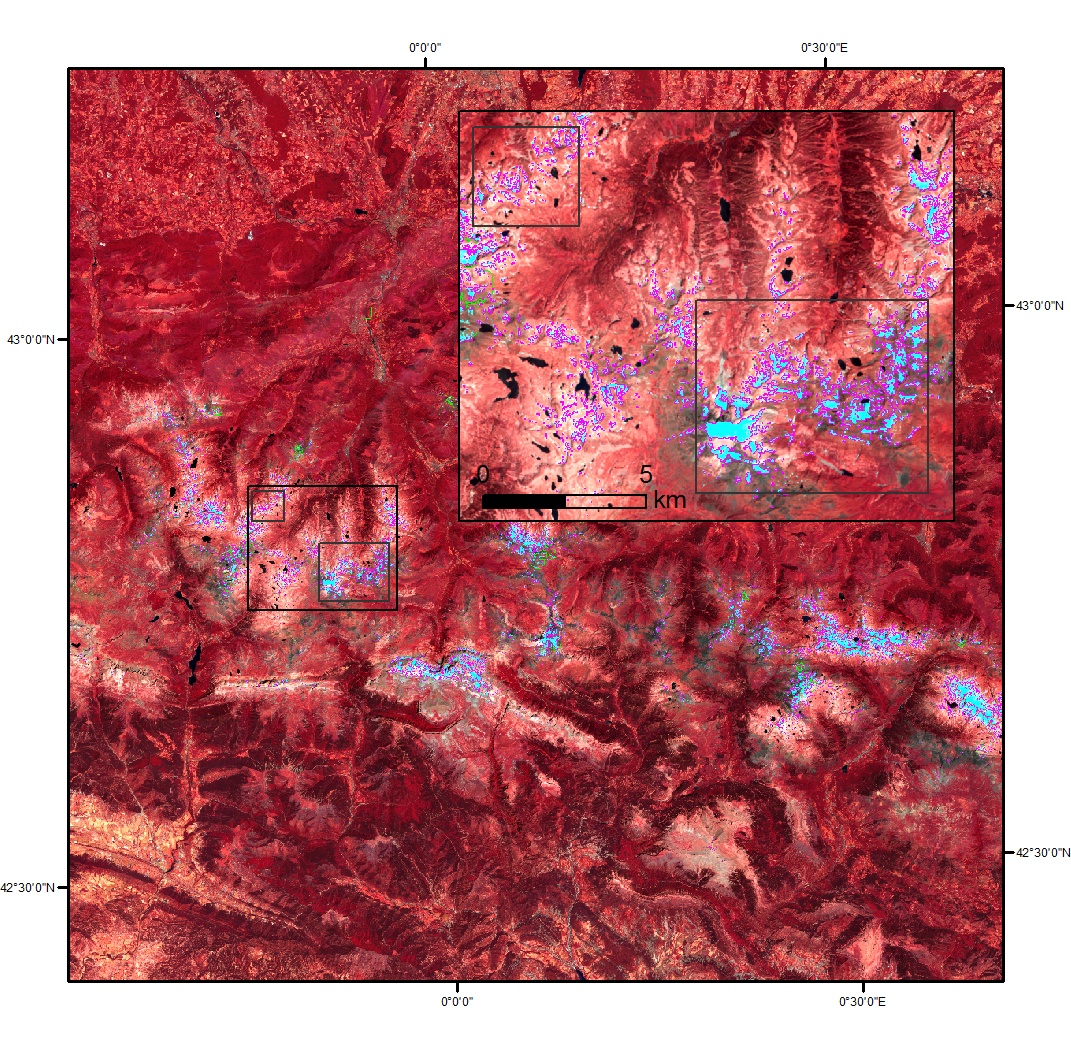
\includegraphics[width=\textwidth]{./images/S2snow.png}
 % S2snow.png: 1071x1048 pixel, 150dpi, 18.13x17.74 cm, bb=0 0 514 503
 \caption{The Sentinel-2A image of 06-July-2015 (level 2A, tile 30TYN) and the snow mask generated by LIS. The snow mask is in magenta and the background image is a color composite RGB NIR/Red/Green. The inset is a zoom in the Vignemale area (Fig.~\ref{fig:S2snowzoom}).}
 \label{fig:S2snow}
\end{figure}

\begin{figure}[h]
 \centering
 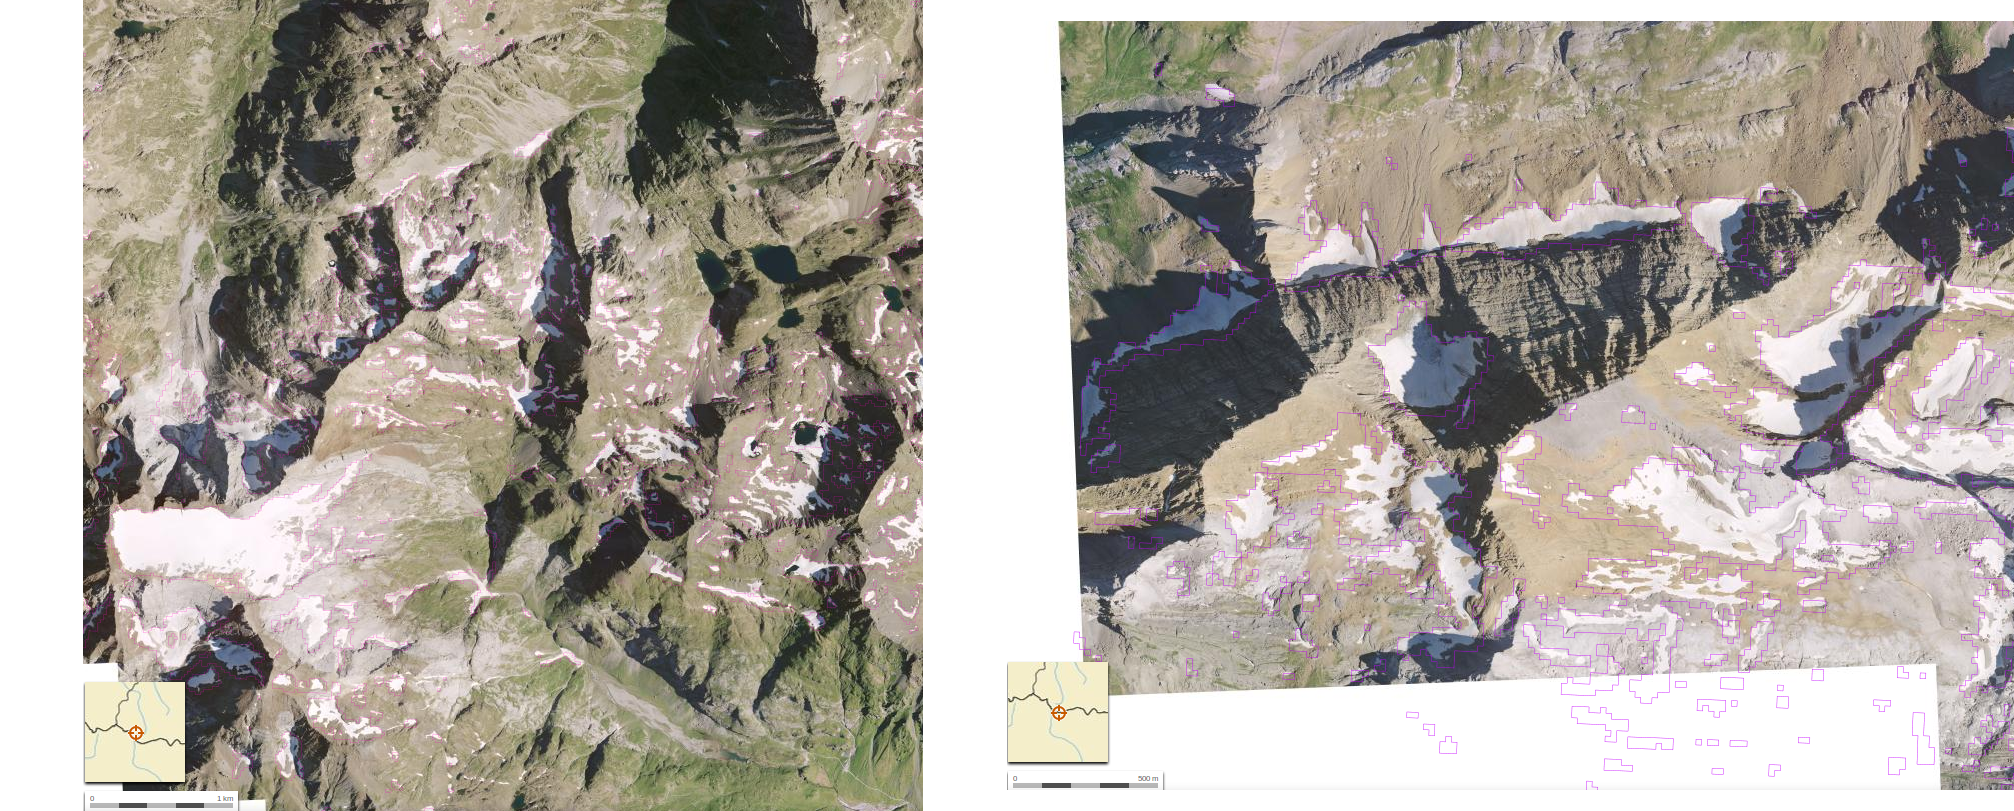
\includegraphics[width=\textwidth]{./images/Sentinel2_testmontage.png}
 % Sentinel2_testmontage.png: 2014x811 pixel, 72dpi, 71.05x28.61 cm, bb=0 0 2014 811
 \caption{The LIS snow mask from the Sentinel-2A image of 06-July-2015 (Fig.~\ref{fig:S2snow}) is superposed to an aerial orthophoto taken in August 2013 and distributed by the Institut National Information Géographique Forestière.}
 \label{fig:S2snowzoom}
\end{figure}

The output of LIS was also examined by comparing the output snow mask from two images acquired on the same day by two different sensors. The example shown in Fig.~\ref{fig:L8vsS4-23042013} illustrates that both snow masks are consistent, although further inspection revealed that the SPOT-4 snow mask tends to underestimate the snow cover area in this case. This is probably due to the lower radiometric resolution of SPOT-4 sensor.

\begin{figure}[h]
 \centering
 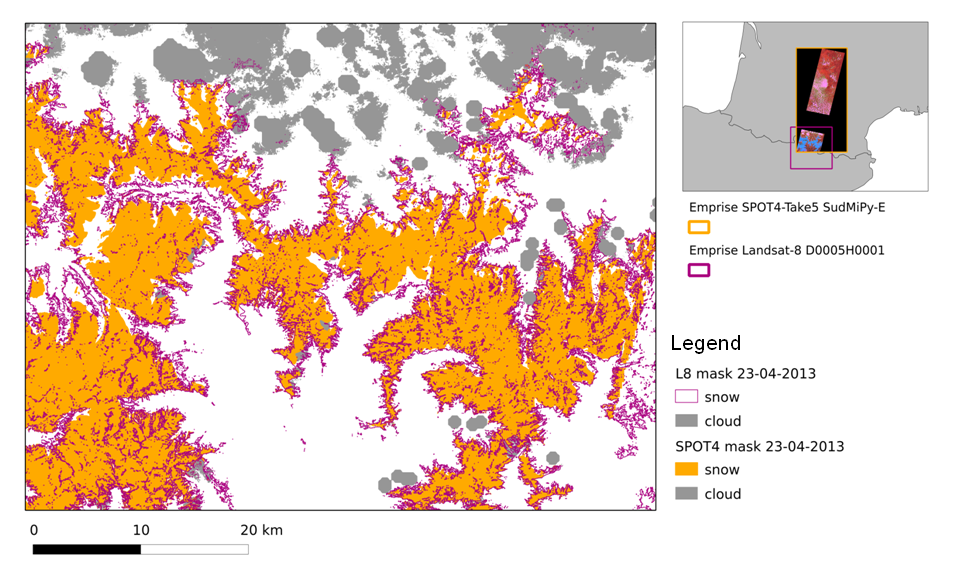
\includegraphics[width=\textwidth]{./images/L8vsS4-23042013_montage.png}
 % L8vsS4-23042013_montage.png: 960x563 pixel, 96dpi, 25.40x14.89 cm, bb=0 0 720 422
 \caption{Comparison of the output of LIS from two a Landsat-8 and SPOT-4 product acquired on the same day.}
 \label{fig:L8vsS4-23042013}
\end{figure}

The output of LIS was also compared to the output of the fmask algorithm\footnote{Zhu, Z., Wang, S. and Woodcock, C.E., 2015. Improvement and expansion of the Fmask algorithm: cloud, cloud shadow, and snow detection for Landsats 4–7, 8, and Sentinel 2 images. Remote Sensing of Environment, 159, pp.269-277.} available in Google Earth Engine (Landsat TOA with Fmask collections). The snow mask are similar, because the method of detection is also based on the NDSI. We found that fmask falsely detects water area in snow-free shaded slopes (an example is given in Fig~\ref{fig:fmask}). The cloud mask is also more conservative than LIS, which is normal given that fmask is a general-purpose algorithm like MACCS. 

\begin{figure}[h]
 \centering
 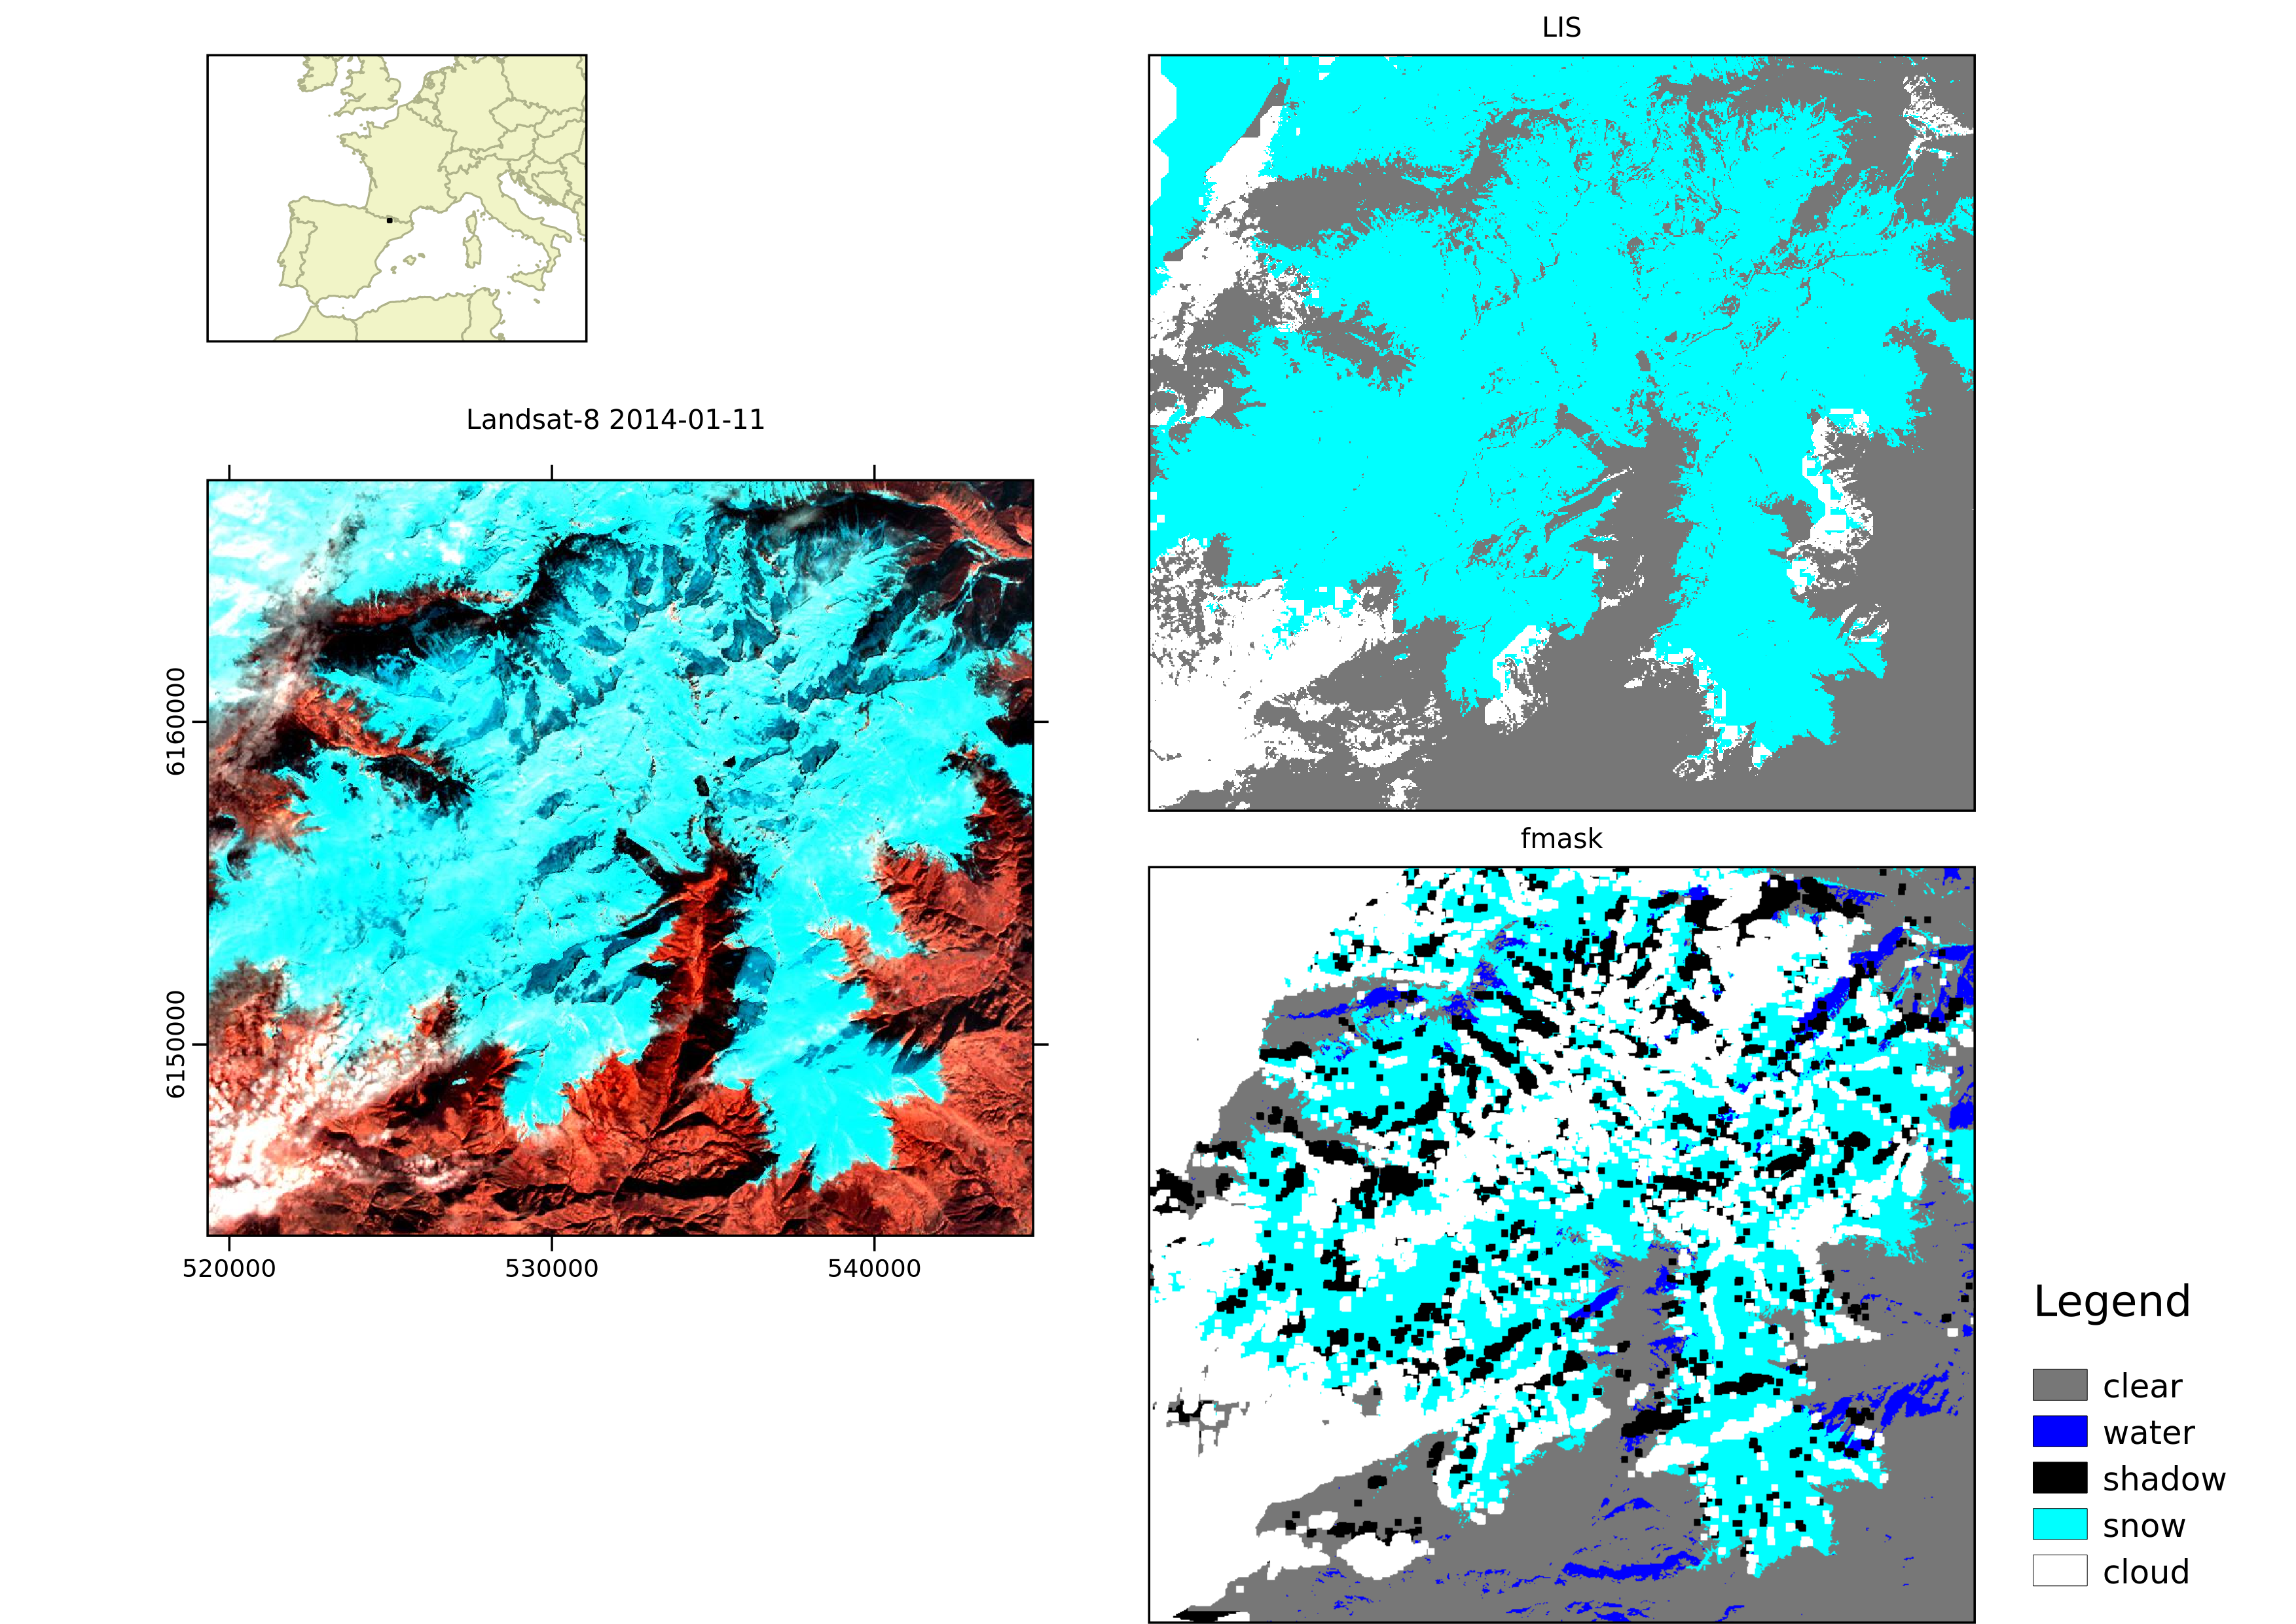
\includegraphics[width=\textwidth]{./images/fmask20140111.png}
 % fmask20140111.png: 3507x2480 pixel, 300dpi, 29.69x21.00 cm, bb=0 0 842 595
 \caption{Comparison of the output of the LIS and fmask algorithm on 2014-01-11 in the Pyrenees.}
 \label{fig:fmask}
\end{figure}


\clearpage

\section{Conclusion and perspectives}\label{par:conclu}

The LIS processing chain is a robust and numerically efficient tool to generate a new, high-resolution snow cover product for Theia Land data center. The LIS snow mask is an improvement from the L2A snow mask (Fig.~\ref{fig:L2AvsLIS}), but its accuracy is largely due to the quality of the slope-corrected L2A product. After the launch of Sentinel-2B the frequency of observations will increase. This will improve the atmospheric corrections by the multi-temporal algorithm MACCS and all the products that are derived from the L2A product in general, including this snow cover extent product. 

\begin{figure}[h]
 \centering
 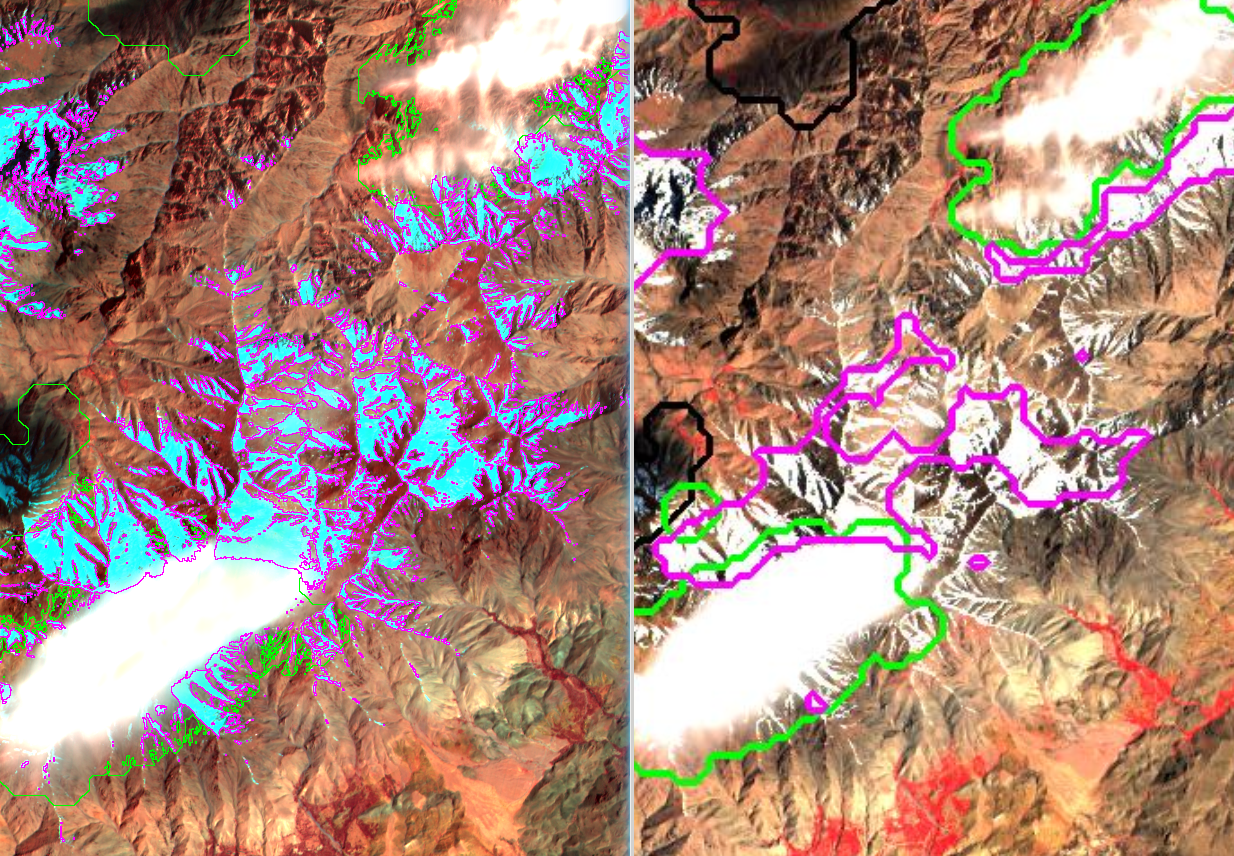
\includegraphics[width=\textwidth]{./images/Maroc_20130327_S4T5.png}
 % Maroc_20130327_S4T5.png: 1234x856 pixel, 85dpi, 36.88x25.58 cm, bb=0 0 1045 725
 \caption{Snow and cloud mask after processing by LIS (left) vs. L2A original cloud and snow mask (right). Clouds are marked in green, cloud shadows in black, snow in magenta. Revisiting the cloud mask enables to increase the area of snow/no snow detection.}
 \label{fig:L2AvsLIS}
\end{figure}


In the meantime we would like to further validate LIS using terrestrial time lapse images in the next year. This could also allow a calibration of the parameters (e.g. $n_2$ ,$r_2$). 

A cloud-free snow cover extent product would facilitate the exploitation of the data by end-users. We plan to work on the development of a cloud-free snow cover product (i.e. a level 3 product). The cloud removal or ``gap-filling'' algorithm will rely on a series a spatio-temporal filters to reclassify the cloud pixels that are output by LIS. This type of gap-filling algorithm was already developed for MODIS snow cover products\footnote{Gascoin, S., Hagolle, O., Huc, M., Jarlan, L., Dejoux, J.-F., Szczypta, C., Marti, R., and Sánchez, R.: A snow cover climatology for the Pyrenees from MODIS snow products, Hydrol. Earth Syst. Sci., 19, 2337-2351.} but must be further assessed on Sentinel-2 time series. We also plan to evaluate the combination of Sentinel-2 and Landsat-8 snow maps to increase the number of observations used by the gap-filling algorithm. 

\clearpage

\appendix

% % This LaTeX was auto-generated from MATLAB code.
% % To make changes, update the MATLAB code and republish this document.
% 
% \documentclass{article}
% \usepackage{graphicx}
% \usepackage{color}
% 
% \sloppy
% \definecolor{lightgray}{gray}{0.5}
% \setlength{\parindent}{0pt}
% 
% \begin{document}

    
    
\section{Test script (castest\_CESneige.m)}\label{par:castest}

\begin{par}
\textbf{Author: Simon Gascoin (CNRS/CESBIO)}
\end{par} \vspace{1em}
\begin{par}
\textbf{June 2015}
\end{par} \vspace{1em}
\begin{par}
This code is a demonstrator of the snow detection algorithm for Sentinel-2 images. It calls the function S2snow (appendix~\ref{par:s2snow}) using subsets of SPOT-4 or Landsat-8 level 2A images.
\end{par} \vspace{1em}
\begin{par}
The input files were generated from L2 images downloaded from Theia Land and pre-processed by three shell scripts:
\end{par} \vspace{1em}
\begin{enumerate}
\setlength{\itemsep}{-1ex}
   \item \texttt{decompresse\_*.sh},        to unzip the files
   \item \texttt{decoupe\_*.sh},        to extract a rectangle AOI from L2A data using       gdal\_translate with projection window defined in the ascii file       \textit{AOI\_test\_CESNeige.csv}
   \item \texttt{projette\_mnt\_*.sh},        to project the SRTM DEM and resample at 30m or 20m       (Landsat8 or Take5) over the same AOI. It uses gdalwarp with the       cubicspline option
\end{enumerate}

\subsection*{Contents}

\begin{itemize}
\setlength{\itemsep}{-1ex}
   \item Configuration
   \item Cloud mask processing parameters
   \item Snow detection parameters
   \item Definition of the input images
   \item Data loading
   \item Snow detection
   \item Figures
\end{itemize}
\begin{par}
Check Matlab version
\end{par} \vspace{1em}
\begin{verbatim}
matlabversion=version;
assert(str2double(matlabversion(end-5:end-2))>=2014,...
    'Needs Matlab version 2014 and later')
\end{verbatim}


\subsection*{Configuration}

\begin{par}
This demo can run for only one image (option 1) or process several images series from different sites and sensors (option 2)
\end{par} \vspace{1em}
\begin{verbatim}
demotype=1;
\end{verbatim}
\begin{par}
If this flag QL is true the code will output three figures for each image
\end{par} \vspace{1em}
\begin{enumerate}
\setlength{\itemsep}{-1ex}
   \item a bar graph showing the snow fraction per elevation band,
   \item a bar graph showing the snow, cloud and elevation area in m2,
   \item a false color composite image overlaid by snow and cloud masks.
\end{enumerate}
\begin{verbatim}
QL=true;
\end{verbatim}
\begin{par}
Define the output path for the figures
\end{par} \vspace{1em}
\begin{verbatim}
pout='../figures/demo_CESneige';
\end{verbatim}
\begin{par}
Define a label to add to the figure file names
\end{par} \vspace{1em}
\begin{verbatim}
label='ndsipass2_015_cloudpass1_bicubic';
\end{verbatim}


\subsection*{Cloud mask processing parameters}

\begin{par}
Resampling factor to determine the "dark clouds" in the initial cloud mask. Here rf=8 corresponds to a target resolution of 240m for Landsat.
\end{par} \vspace{1em}
\begin{verbatim}
rf=8;
\end{verbatim}
\begin{par}
Dark cloud threshold (reflectance unit: per mil). The clouds pixels with a (coarse) reflectance lower than rRed\_darkcloud are selected to pass the snow test
\end{par} \vspace{1em}
\begin{verbatim}
rRed_darkcloud=500;
\end{verbatim}
\begin{par}
Back to cloud threshold. Pixels which are not detected as snow then they go back to the cloud mask only if their reflectance at full resolution is greater than rRed\_backtocloud. Here we use full resolution reflectances because resampled cloud pixels reflectance drops rapidly along the cloud edges due to the mixing with the land reflectance.
\end{par} \vspace{1em}
\begin{verbatim}
rRed_backtocloud=100;
\end{verbatim}


\subsection*{Snow detection parameters}

\begin{par}
Elevation band height in m.
\end{par} \vspace{1em}
\begin{verbatim}
dz=100;
\end{verbatim}
\begin{par}
NDSI threshold for pass 1
\end{par} \vspace{1em}
\begin{verbatim}
ndsi_pass1=0.4;
\end{verbatim}
\begin{par}
Threshold in the red reflectance for pass 1
\end{par} \vspace{1em}
\begin{verbatim}
rRed_pass1=200;
\end{verbatim}
\begin{par}
NDSI threshold for pass 2
\end{par} \vspace{1em}
\begin{verbatim}
ndsi_pass2=0.15; % Note: Zhu's fmask algorithm uses 0.15
\end{verbatim}
\begin{par}
Threshold in the red reflectance for pass 2
\end{par} \vspace{1em}
\begin{verbatim}
rRed_pass2=120;
\end{verbatim}
\begin{par}
Minimum snow fraction from which to compute the snowline elevation (zs)
\end{par} \vspace{1em}
\begin{verbatim}
fsnow_lim=0.1;
\end{verbatim}
\begin{par}
Snow fraction limit to go to pass 2. The total snow fraction after pass 1 is computed to decide whether or not proceed to pass 2. If the snow fraction is below fsnow\_total\_lim then pass 2 is skipped because the number of snow pixels is not sufficient to properly determine the snow line elevation. Here we use 1000 pixels.
\end{par} \vspace{1em}
\begin{verbatim}
fsnow_total_lim=0.001; % Warning! it depends on the image size
\end{verbatim}


\subsection*{Definition of the input images}

\begin{verbatim}
switch demotype
    case 1
\end{verbatim}
\begin{par}
use only 1 image
\end{par} \vspace{1em}
\begin{verbatim}
        satlist={'Take5'};
        sitelist{1}={'Maroc'};
        datelist{1}{1}={'20130327'}; % format yyyymmdd
\end{verbatim}
\begin{verbatim}
    case 2
\end{verbatim}
\begin{par}
process a batch of 2 x Landsat8 and 4 x Take5 images series
\end{par} \vspace{1em}
\begin{verbatim}
        [satlist,sitelist,datelist]=load_demo_input('all');
\end{verbatim}
\begin{verbatim}
    otherwise
        error('demotype should be 1 or 2')
end
\end{verbatim}


\subsection*{Data loading}

\begin{par}
Begin the sensor loop
\end{par} \vspace{1em}
\begin{verbatim}
nsat=length(satlist);
for isat=1:nsat
\end{verbatim}
\begin{verbatim}
    sat=satlist{isat};

    nsite=length(sitelist{isat});
\end{verbatim}
\begin{par}
Get the sensor band numbers and no-data value
\end{par} \vspace{1em}
\begin{verbatim}
    switch sat
        case 'Take5'
            nGreen=1; % Index of green band
            nMIR=4; % Index of SWIR band (1 to 3 µm) = band 11 (1.6 µm) in S2
            nRed=2; % Index of red band
            nodata=-10000; % no-data value
        case 'Landsat8'
            nGreen=3;
            nMIR=6;
            nRed=4;
            nodata=-10000;
        otherwise
            error('sat should be Take5 or Landsat8')
    end
\end{verbatim}
\begin{par}
Begin the site loop
\end{par} \vspace{1em}
\begin{verbatim}
    for isite=1:nsite;
\end{verbatim}
\begin{verbatim}
        site=sitelist{isat}{isite};
        ndate=length(datelist{isat}{isite});
\end{verbatim}
\begin{par}
read SRTM DEM for this site
\end{par} \vspace{1em}
\begin{verbatim}
        fdem=['../' sat '/AOI_test_CESNeige/SRTM/' site '/' site '.tif'];
        [Zdem,R]=geotiffread(fdem);
\end{verbatim}
\begin{par}
Begin the date loop
\end{par} \vspace{1em}
\begin{verbatim}
        for idate=1:ndate
\end{verbatim}
\begin{verbatim}
            date=datelist{isat}{isite}{idate};
\end{verbatim}
\begin{par}
Read the L2 reflectance data (search the image filename based on the date)
\end{par} \vspace{1em}
\begin{verbatim}
            pL2=['../' sat '/AOI_test_CESNeige/LEVEL2A/' site]; % path
            fL2=dir([pL2 '/*' date '*PENTE*.TIF']); % file list
            assert(~isempty(fL2),'The L2 image is not present in the input directory')
            f=[pL2 '/' fL2.name];
            [ZL2,~]=geotiffread(f);
\end{verbatim}
\begin{par}
The data are converted to double because it enables to work with NaN, but we could probably avoid this to optimize memory use..
\end{par} \vspace{1em}
\begin{verbatim}
            ZL2=double(ZL2);
            ZL2(ZL2==nodata)=NaN;
\end{verbatim}
\begin{par}
Read the cloud mask
\end{par} \vspace{1em}
\begin{verbatim}
            fc=dir([pL2 '/*' date '*NUA.TIF']);
            assert(~isempty(fc),'The cloud mask is not present in the input directory')
            f=[pL2 '/' fc.name];
            [Zc,~]=geotiffread(f);
\end{verbatim}


\subsection*{Snow detection}

\begin{par}
Calls the function S2snow (appendix~\ref{par:s2snow})
\end{par} \vspace{1em}
\begin{verbatim}
            [snowtest,cloudtestfinal,z_center,B1,B2,fsnow,zs,...
                fsnow_z,fcloud_z,N,z_edges]...
                = S2snow(...
                ZL2,Zc,Zdem,nGreen,nRed,nMIR,rf,QL,rRed_darkcloud,...
                ndsi_pass1,ndsi_pass2,rRed_pass1,rRed_pass2,dz,fsnow_lim,...
                fsnow_total_lim,rRed_backtocloud);
\end{verbatim}


\subsection*{Figures}

\begin{verbatim}
            if QL
\end{verbatim}
\begin{par}
Draw a bar plot of the snow fraction per elevation band
\end{par} \vspace{1em}
\begin{verbatim}
                figure(1),clf
                barh(z_center,fsnow_z,1,'facecolor','c');
                hold on
                if ~isempty(zs)
                    hrf=refline(0,zs);
                    set(hrf,'Color','r','LineStyle','--','LineWidth',2)
                end
                xlabel('Fractional area')
                ylabel('Elevation (m)')
                legend('Snow','zs')
                title(sprintf('%s zs=%g',date,zs))
\end{verbatim}

%         \color{lightgray} \begin{verbatim}Warning: MATLAB has disabled some advanced graphics rendering features by
% switching to software OpenGL. For more information, click <a
% href="matlab:opengl('problems')">here</a>. 
% \end{verbatim} \color{black}
    
\includegraphics [width=4in]{include/castest_CESneige_01.eps}
\begin{par}
Draw a bar plot of the snow area and elevation band area
\end{par} \vspace{1em}
\begin{verbatim}
                figure(2),clf
                [Nz,~,~] = histcounts(Zdem(:),z_edges);
                barh(z_center,Nz,1,'facecolor',.8*[1 1 1]);
                hold on
                barh(z_center,(fcloud_z+fsnow_z).*Nz',1,'facecolor',.5*[1 1 1]);
                barh(z_center,fsnow_z.*Nz',1,'facecolor','c');
                if ~isempty(zs)
                    hrf=refline(0,zs);
                    set(hrf,'Color','r','LineStyle','--','LineWidth',2)
                end
                xlabel('Area (m2)')
                ylabel('Elevation (m)')
                legend('DEM','Cloud','Snow','zs')
                title(sprintf('%s zs=%g',date,zs))
\end{verbatim}

\includegraphics [width=4in]{include/castest_CESneige_02.eps}
\begin{par}
Show an RGB composition overlaid with pass 1 and 2 snow cover polygons. The clouds pixels are in black.
\end{par} \vspace{1em}
\begin{verbatim}
                figure(3),clf
                z=ZL2(:,:,[nMIR nRed nGreen]);
                max_b=[300 300 300];
                z2=zeros(size(z),'uint8');
                for b=1:3
                    z2(:,:,b)=~cloudtestfinal.*double(z(:,:,b))/max_b(b)*255;
                end
                imshow(uint8(z2),'Border','tight')
                hold on
                for k = 1:length(B1)
                    boundary = B1{k};
                    %         if length(boundary)>100
                    plot(boundary(:,2), boundary(:,1), 'y', 'LineWidth', 1)
                    %         end
                end
                if ~isempty(zs)
                    for k = 1:length(B2)
                        boundary = B2{k};
                        %         if length(boundary)>100
                        plot(boundary(:,2), boundary(:,1), 'm', 'LineWidth', 1)
                        %         end
                    end
                end
\end{verbatim}

%         \color{lightgray} \begin{verbatim}Warning: Image is too big to fit on screen; displaying at 67% 
% \end{verbatim} \color{black}
    
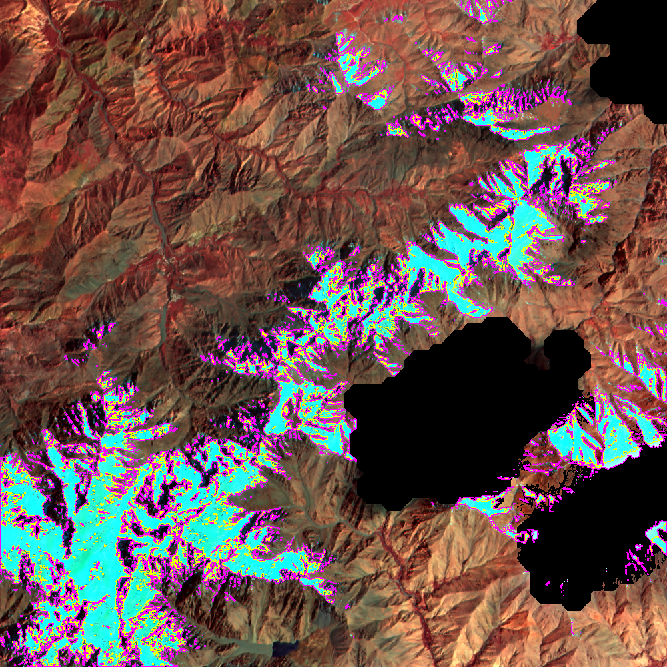
\includegraphics [width=4in]{include/castest_CESneige_03.eps}
\begin{par}
Print figures
\end{par} \vspace{1em}
\begin{verbatim}
                set(1:3,'PaperPositionMode','auto','Visible','off');
                pfig=[pout '/' sat '/' site];
                system(sprintf('mkdir -p %s/zs1',pfig));
                system(sprintf('mkdir -p %s/zs2',pfig));
                system(sprintf('mkdir -p %s/QL',pfig));
                f1=sprintf('%s/zs1/%s_%s_%s_%s.png',pfig,sat,site,date,label);
                f2=sprintf('%s/zs2/%s_%s_%s_%s.png',pfig,sat,site,date,label);
                f3=sprintf('%s/QL/%s_%s_%s_%s.png',pfig,sat,site,date,label);
                print(1,f1,'-dpng')
                print(2,f2,'-dpng')
                print(3,f3,'-dpng')
\end{verbatim}
\begin{verbatim}
            end
\end{verbatim}
\begin{verbatim}
        end
\end{verbatim}
\begin{verbatim}
    end
\end{verbatim}
\begin{verbatim}
end
\end{verbatim}



% \end{document}
    

% 
% % This LaTeX was auto-generated from MATLAB code.
% % To make changes, update the MATLAB code and republish this document.
% 
% \documentclass{article}
% \usepackage{graphicx}
% \usepackage{color}
% 
% \sloppy
% \definecolor{lightgray}{gray}{0.5}
% \setlength{\parindent}{0pt}
% 
% \begin{document}

    
    
\section{Snow detection function (S2snow.m)}\label{par:s2snow}

\begin{par}
\textbf{Author: Simon Gascoin (CNRS/CESBIO)}
\end{par} \vspace{1em}
\begin{par}
\textbf{June 2015}
\end{par} \vspace{1em}
\begin{par}
This function computes the snow presence and absence (snow/no-snow) from a high-resolution optical multispectral image like Sentinel-2 (eg Landsat-8, SPOT-4) The input are the full resolution reflectances corrected from atmospheric and slope effects (Level 2A), the associated cloud mask and a digital elevation model. The output is a mask with three classes: snow/no-snow/cloud. The output cloud mask is different from the input cloud mask.
\end{par} \vspace{1em}
\begin{par}
The snow detection algorithm works in two passes: first the most evident snow is detected using a set of conservative thresholds, then this snow pixels are used to determine the lower elevation of the snow cover. A second pass is performed for the pixels above this elevation with a new set of less conservative thresholds
\end{par} \vspace{1em}
\begin{par}
The snow detection is made on a pixel-basis using the Normalized Difference Snow Index (NDSI):
\end{par} \vspace{1em}
\begin{par}
$$ \textrm{NDSI} = \frac{\rho_\textrm{{Green}}-\rho_\textrm{{MIR}}}{\rho_\textrm{{Green}}+\rho_\textrm{{MIR}}} $$
\end{par} \vspace{1em}
\begin{par}
where $\rho_\textrm{{Green}}$ is the reflectance in the green channel and $\rho_\textrm{{Green}}$ in the shortwave infrared.
\end{par} \vspace{1em}

\subsection*{Contents}

\begin{itemize}
\setlength{\itemsep}{-1ex}
   \item Function call
   \item Inputs
   \item Outputs
   \item Initial cloud mask processing
   \item Pass 1 : first snow test
   \item Pass 2 : second snow test
   \item Final update of the cloud mask
\end{itemize}


\subsection*{Function call}

\begin{verbatim}
function [snowtest,cloudtestfinal,z_center,B1,B2,fsnow,zs,...
    fsnow_z,fcloud_z,N,z_edges]...
    = S2snow(...
    ZL2,Zc,Zdem,nGreen,nRed,nMIR,rf,QL,rRed_darkcloud,...
    ndsi_pass1,ndsi_pass2,rRed_pass1,rRed_pass2,dz,fsnow_lim,...
    fsnow_total_lim,rRed_backtocloud)
\end{verbatim}


\subsection*{Inputs}

\begin{itemize}
\setlength{\itemsep}{-1ex}
   \item ZL2: L2A reflectances (NxMxB double array, where B is the number of band)
   \item Zc: cloud mask (Zc\ensuremath{>}0 is cloud) (NxM array)
   \item Zdem: digital elevation model (NxM array)
   \item nGreen, nRed, nMIR: index of green, red, SWIR band in ZL2
   \item rf: resampling factor for cloud reflectance
   \item QL: quicklooks? (boolean)
   \item ndsi\_pass1,ndsi\_pass2,rRed\_pass1,rRed\_pass2,rRed\_backtocloud: parameters for reflectance-based tests (see the documentation in appendix~\ref{par:castest})
   \item dz: elevation band width
   \item fsnow\_lim: minimum snow fraction in an elevation band to define zs
   \item fsnow\_total\_lim: minimum snow fraction in the whole image after pass1 to go to pass2
\end{itemize}


\subsection*{Outputs}

\begin{itemize}
\setlength{\itemsep}{-1ex}
   \item snowtest: snow presence/absence (NxM boolean)
   \item cloudtestfinal: cloud presence/absence (NxM boolean)
   \item z\_center: centers of the elevation bands (vector)
   \item B1, B2: snow cover contours after pass 1 and pass 2 (cell)
   \item fsnow: total snow fraction in the image after pass 1
   \item zs: snow elevation for pass 2
   \item fsnow\_z: snow fraction in each band
   \item N: number of clear pixels in each elevation band
   \item z\_edges: upper and lower limits of the elevation bands
\end{itemize}


\subsection*{Initial cloud mask processing}

\begin{par}
The L2A cloud mask is too conservative and much useful information for snow cover mapping is lost.
\end{par} \vspace{1em}
\begin{par}
We allow the reclassification of some cloud pixels in snow or no-snow only if they have a rather low reflectance. We select only these "dark clouds" because the NDSI test is robust to the snow/cloud confusion in this case
\end{par} \vspace{1em}
\begin{par}
Initial cloud mask (incl. cloud shadows)
\end{par} \vspace{1em}
\begin{verbatim}
cloudtestinit = Zc>0;
\end{verbatim}

%         \color{lightgray} \begin{verbatim}Error using S2snow (line 72)
% Not enough input arguments.
% \end{verbatim} \color{black}
    \begin{par}
Get the cloud shadows
\end{par} \vspace{1em}
\begin{verbatim}
code_shad = bin2dec(fliplr('00000011'));
cloudshadow = bitand(Zc,code_shad)>0;
\end{verbatim}
\begin{par}
We exclude high clouds detected from with 1.38 µm band (S2 and L8 only)
\end{par} \vspace{1em}
\begin{verbatim}
code_highcloud = bin2dec(fliplr('00000100'));
highcloud = bitand(Zc,code_highcloud)>0;
\end{verbatim}
\begin{par}
The "dark cloud" are found with a threshold rRed\_darkcloud in the red band after bilinear resampling of the original image to match the MACCS algorithm philosophy but the benefit of this was not yet evaluated.
\end{par} \vspace{1em}
\begin{verbatim}
rRedcoarse = imresize(ZL2(:,:,nRed), 1/rf,'bicubic');
\end{verbatim}
\begin{par}
Then we oversample to the initial resolution using nearest neighbour to have the same image size.
\end{par} \vspace{1em}
\begin{verbatim}
rRedcoarse_oversampl = imresize(rRedcoarse,rf,'nearest');
\end{verbatim}
\begin{par}
clear rRedcoarse to free up memory
\end{par} \vspace{1em}
\begin{verbatim}
clear rRedcoarse
\end{verbatim}
\begin{par}
These pixels are removed from the intial cloud mask unless they were flagged as a cloud shadow or high cloud. The snow detection will not be applied where cloudtesttmp is true.
\end{par} \vspace{1em}
\begin{verbatim}
cloudtesttmp = ...
    (cloudtestinit & rRedcoarse_oversampl>rRed_darkcloud)...
    | cloudshadow | highcloud;
\end{verbatim}


\subsection*{Pass 1 : first snow test}

\begin{par}
The test is based on the Normalized Difference Snow Index (ndsi0) and the reflectance value in the red channel
\end{par} \vspace{1em}
\begin{verbatim}
ndsi0 = (ZL2(:,:,nGreen)-ZL2(:,:,nMIR))./(ZL2(:,:,nGreen)+ZL2(:,:,nMIR));
\end{verbatim}
\begin{par}
A pixel is marked as snow covered if NDSI is higher than ndsi\_pass1 and if the red reflectance is higher than Red\_pass1
\end{par} \vspace{1em}
\begin{verbatim}
snowtest = ~cloudtesttmp & ndsi0>ndsi_pass1 & ZL2(:,:,nRed)>rRed_pass1;
\end{verbatim}
\begin{par}
Now we can update the cloud mask Some pixels were originally marked as cloud but were not reclassified as snow after pass 1. These pixels are marked as cloud if they have a high reflectance ("back to black"). Otherwise we keep them as "no-snow" ("stayin alive").
\end{par} \vspace{1em}
\begin{verbatim}
cloudtestpass1 = cloudtesttmp ...
    | (~snowtest & cloudtestinit & ZL2(:,:,nRed)>rRed_backtocloud);
\end{verbatim}
\begin{par}
For the quicklooks we compute the boundary of the snow cover after pass 1.
\end{par} \vspace{1em}
\begin{par}
\textit{Warning this uses much computer time.}
\end{par} \vspace{1em}
\begin{verbatim}
if QL
    [B1, ~] = bwboundaries(snowtest); % requires Matlab Image Processing Toolbox
else
    B1 = [];
end
\end{verbatim}
\begin{par}
Initialize some output variables as empty array in case they is not reached in pass 2
\end{par} \vspace{1em}
\begin{verbatim}
B2 = [];
zs = [];
N = [];
bin = [];
\end{verbatim}


\subsection*{Pass 2 : second snow test}

\begin{par}
Based on the DEM, the scene is discretized in elevation band of height dz. The elevation bands start from the minimal elevation found in the DEM resampled at the image resolution. The edges of elevation band are :
\end{par} \vspace{1em}
\begin{verbatim}
z_edges = double(min(Zdem(:)):dz:max(Zdem(:)));

% NB) the colon operator j:i:k is the same as [j,j+i,j+2i, ...,j+m*i],
% where m = fix((k-j)/i).
\end{verbatim}
\begin{par}
The number of bins is :
\end{par} \vspace{1em}
\begin{verbatim}
nbins = length(z_edges)-1;
\end{verbatim}
\begin{par}
The mean elevation of each band is computed for the graphics but not used by the algorithm
\end{par} \vspace{1em}
\begin{verbatim}
z_center = mean([z_edges(2:end);z_edges(1:end-1)]);
\end{verbatim}
\begin{par}
The lower edge of each bin is used to define zs
\end{par} \vspace{1em}
\begin{verbatim}
z_loweredges=z_edges(1:end-1);
\end{verbatim}
\begin{par}
We get the number of pixels (N) which are cloud-free (at this step) in each bin, and the index array (bin) to identify the elevation band corresponding to a pixel in the cloud-free portion of the image
\end{par} \vspace{1em}
\begin{verbatim}
if nbins>0
    [N,~,bin] = histcounts(Zdem(~cloudtestpass1),z_edges);
end
\end{verbatim}
\begin{par}
Compute the fraction of snow pixels in each elevation band
\end{par} \vspace{1em}
\begin{verbatim}
fsnow_z = zeros(nbins,1);
fcloud_z = zeros(nbins,1);
if ~isempty(bin)
\end{verbatim}
\begin{par}
We collect the snow pixels only in the cloud free areas
\end{par} \vspace{1em}
\begin{verbatim}
    M = snowtest(~cloudtestpass1(:)); % this also reshapes snowtest from a
    % 2D array to 1D array to match the bin index array dimension
\end{verbatim}
\begin{par}
Then we start to loop over the each elevation band
\end{par} \vspace{1em}
\begin{verbatim}
    for i = 1:nbins
\end{verbatim}
\begin{par}
We sum the snow pixels and divide by the number of cloud-free pixels
\end{par} \vspace{1em}
\begin{verbatim}
        if N(i)>0
            fsnow_z(i) = sum(M(bin==i))/N(i);
            fcloud_z(i) = sum(cloudtestpass1(bin==i))/N(i);
        else
            fsnow_z(i) = NaN;
            fcloud_z(i) = NaN;
        end
\end{verbatim}
\begin{verbatim}
    end
\end{verbatim}
\begin{par}
We compute the total fraction of snow pixels in the image
\end{par} \vspace{1em}
\begin{verbatim}
    fsnow = nnz(snowtest)/numel(snowtest);
\end{verbatim}
\begin{par}
The pass 2 snow test is not performed if there is not enough snow detected in pass 1.
\end{par} \vspace{1em}
\begin{verbatim}
    if fsnow>fsnow_total_lim
\end{verbatim}
\begin{par}
We get zs, the minimum snow elevation above which we apply pass 2. zs is \textbf{two elevation bands} below the band at which fsnow \ensuremath{>} fsnow\_lim
\end{par} \vspace{1em}
\begin{verbatim}
        izs = find(fsnow_z>fsnow_lim,1,'first');
        zs = z_loweredges(max(izs-2,1));
\end{verbatim}
\begin{verbatim}
    end
\end{verbatim}
\begin{verbatim}
end
\end{verbatim}
\begin{par}
if zs was found then we apply the second snow test : A pixel is marked as snow covered if NDSI is higher than ndsi\_pass2 and if the red reflectance is higher than Red\_pass1... and if it is above zs!
\end{par} \vspace{1em}
\begin{verbatim}
if ~isempty(zs)
\end{verbatim}
\begin{verbatim}
    snowtest2 = ~cloudtesttmp ... % we use cloudtesttmp again
        & ndsi0>ndsi_pass2 ...
        & Zdem>zs ...
        & ZL2(:,:,nRed)>rRed_pass2;
\end{verbatim}
\begin{par}
We add these snow pixels in the snow mask from pass 1
\end{par} \vspace{1em}
\begin{verbatim}
    snowtest = snowtest2 | snowtest;
\end{verbatim}
\begin{par}
For the quicklooks we compute the boundary of the snow cover after pass 2 \textit{Warning this uses much computer time.}
\end{par} \vspace{1em}
\begin{verbatim}
    if QL
        [B2, ~] = bwboundaries(snowtest);
    end
\end{verbatim}
\begin{verbatim}
end
\end{verbatim}


\subsection*{Final update of the cloud mask}

\begin{par}
Some pixels were originally marked as cloud but were not reclassified as snow after pass 1. These pixels are marked as cloud if they have a high reflectance ("back to black"). Otherwise we keep them as "no-snow" ("stayin alive").
\end{par} \vspace{1em}
\begin{verbatim}
cloudtestfinal = cloudtesttmp ...
    | (~snowtest & cloudtestinit & ZL2(:,:,nRed)>rRed_backtocloud);
\end{verbatim}



% \end{document}
    

\end{document}
